\documentclass{oci}
\usepackage[utf8]{inputenc}
\usepackage{lipsum}

\title{Partido de ping-pong}

\begin{document}
\begin{problemDescription}
  \begin{center}
    \vskip -1em
    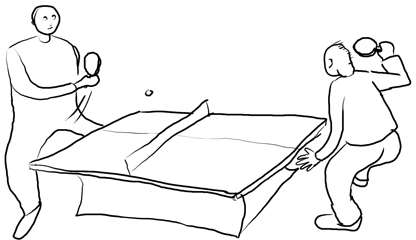
\includegraphics[scale=0.4]{ping-pong.jpg}
  \end{center}
 Jota Pe y Nelman son fanáticos del ping-pong.
Cada vez que se juntan aprovechan de jugar un partido.
Sus partidos no son profesionales y siguen las siguientes reglas que ellos mismos han inventado:
\begin{itemize}
  \item El partido se juega a $N$ puntos y el primero que llega a los $N$ puntos gana.
  \item La cantidad de puntos, es decir, el valor de $N$, puede ser distinto en cada partido.
  \item En cada partido uno de los dos comienza sacando.
  \item Cada jugador conserva su saque hasta perder un punto.
\end{itemize}

Lo que no saben Jota Pe y Nelman es que sus partidos son muy predecibles.
Resulta que cada vez que a Jota Pe le toca sacar tiene una racha de $A$ puntos, es decir, gana $A$ puntos seguidos y luego pierde el saque.
Lo mismo pasa con Nelman, cada vez que a él le toca sacar tiene una racha de $B$ puntos y luego pierde su saque.
El largo de las rachas, es decir, el valor de $A$ y $B$, depende del día en que jueguen.

Jota Pe y Nelman quedarían muy sorprendidos si alguien fuera capaz de adivinar quién de los dos va a ganar un partido antes de que lo jueguen.
>Qué tal si haces un programa para sorprenderlos?
\end{problemDescription}

\begin{inputDescription}
  La entrada está compuesta de dos líneas.

  La primera línea contiene dos enteros $N$ y $P$.
  $N$ corresponde a la cantidad de puntos a los que se jugará el partido.
  $P$ es un entero que indica quién comenzará sacando (Jota Pe = 1 y Nelman = 2).
  
  La siguiente línea contiene dos enteros $A$ y $B$, que representan respectivamente el largo de las rachas de Jota Pe y de Nelman.
\end{inputDescription}

\begin{outputDescription}
  Tu programa debe imprimir un 1 si Jota Pe es quién ganará el partido y un 2 si Nelman es quién ganará el partido.
\end{outputDescription}

\begin{scoreDescription}
  \score{100} Este problema tiene solo una subtarea. Se probarán varios casos donde $1 \le N \le 100$ y $1 \le A, B \le N$.
\end{scoreDescription}

\begin{sampleDescription}
% \sampleIO{sample1}
% \sampleIO{sample1}
\end{sampleDescription}

\end{document}